\documentclass[tikz,border=12pt]{standalone}
\usepackage[T1]{fontenc}
\usepackage{mathpazo}
\usepackage{amsmath,amssymb}
\usetikzlibrary{arrows.meta, positioning, calc}

\definecolor{stblue}{HTML}{7B97AD}
\definecolor{rwgold}{HTML}{B8995E}
\definecolor{sage}{HTML}{7A9A7E}
\definecolor{dkbrown}{HTML}{3D3530}
\definecolor{wmgray}{HTML}{7B7067}
\definecolor{cream}{HTML}{F9F6F0}
\definecolor{border}{HTML}{D4C9B8}
\definecolor{terracotta}{HTML}{C47A6A}

\begin{document}
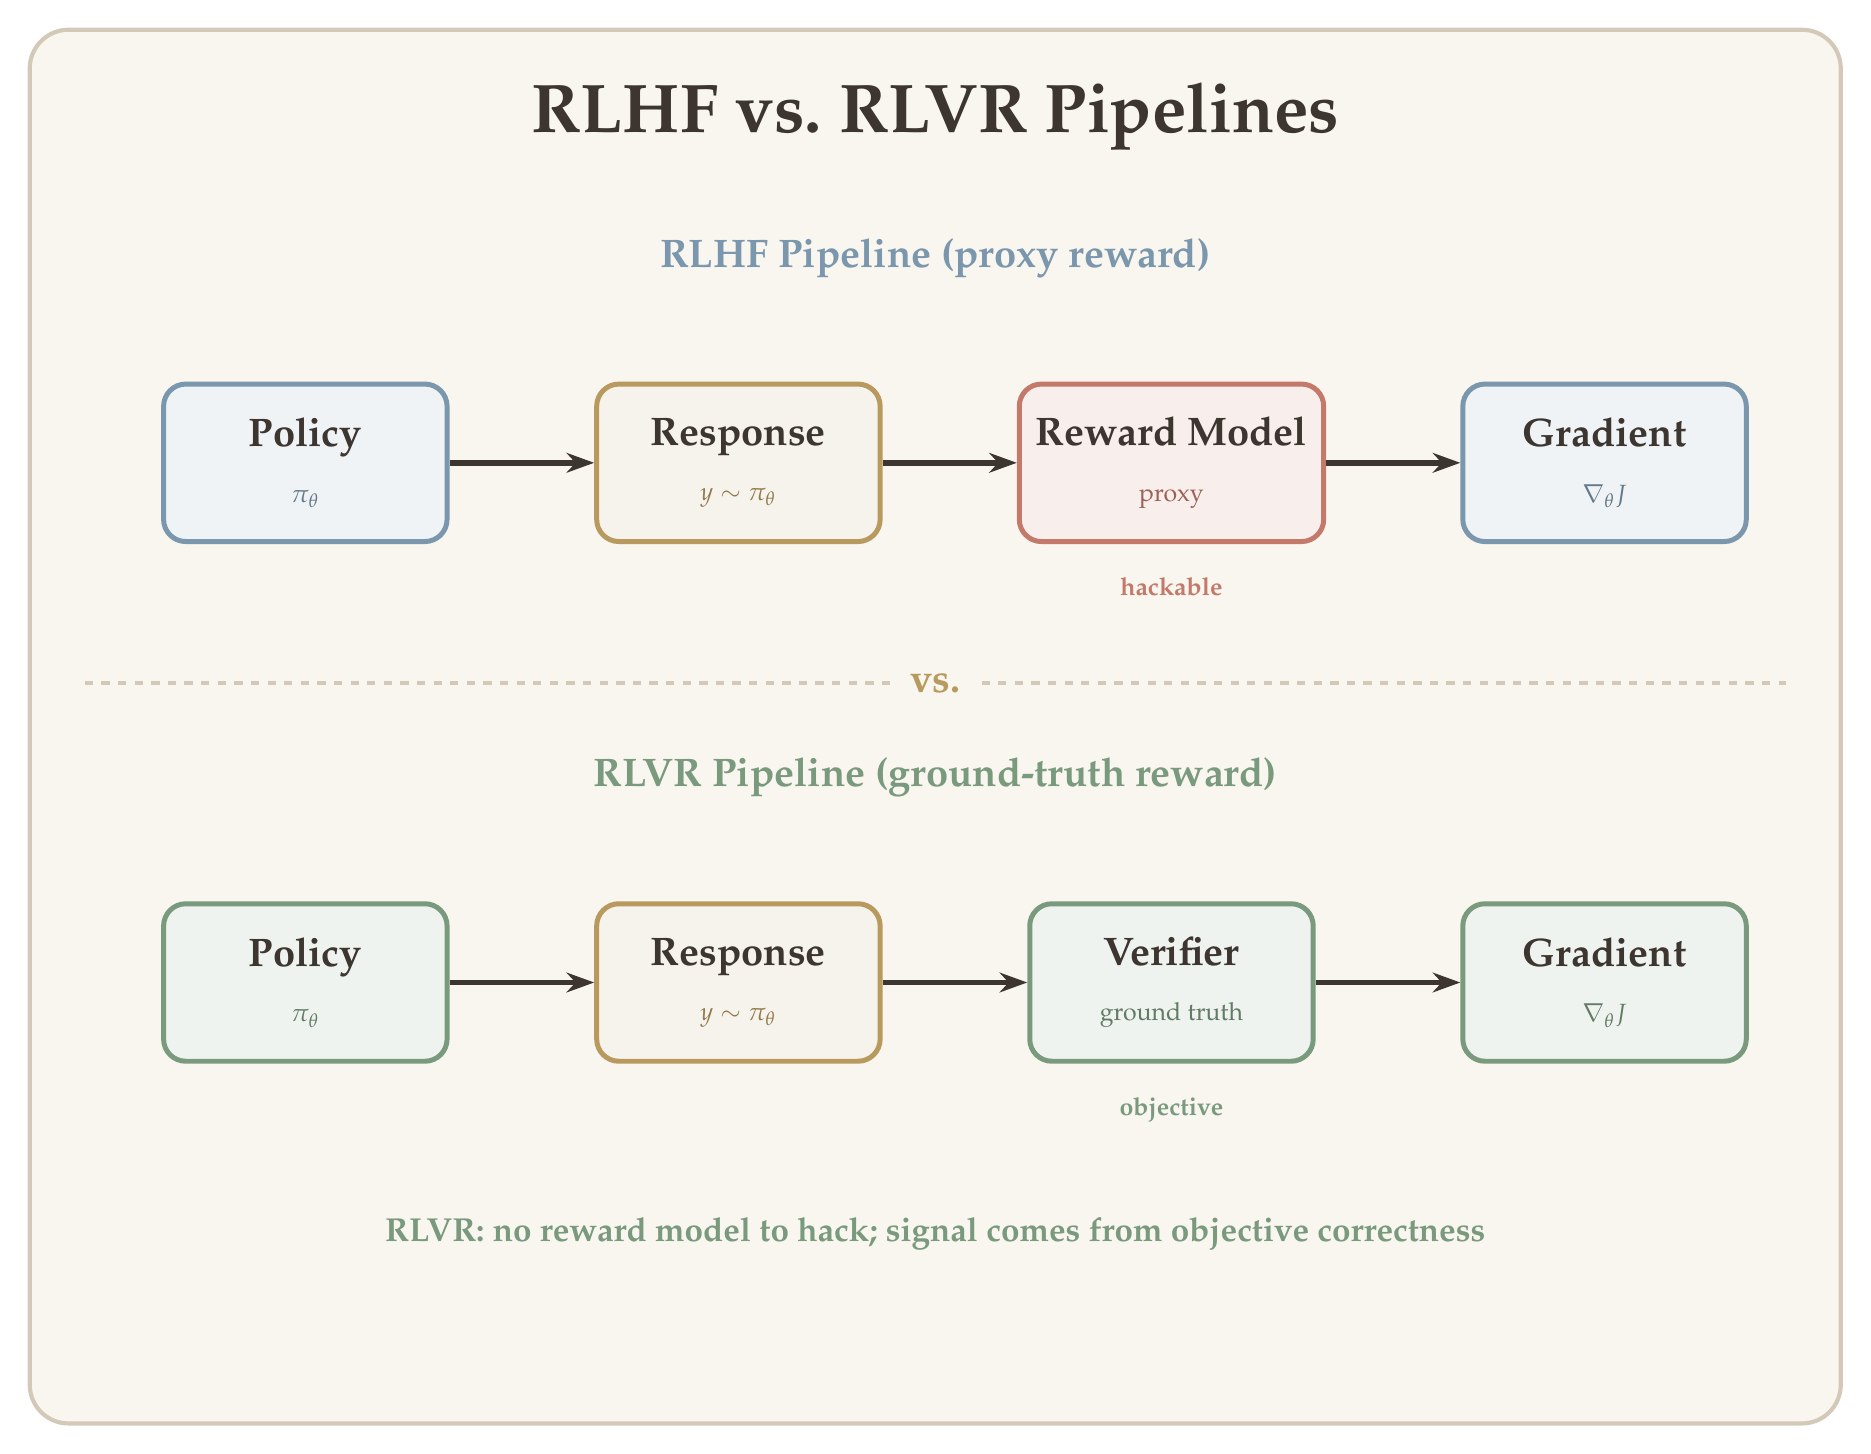
\begin{tikzpicture}[
  >={Stealth[length=3.5mm, width=2.5mm]},
  pipebox/.style 2 args={
    draw=#1, line width=1.8pt, fill=#1!12, rounded corners=8pt,
    minimum width=36mm, minimum height=20mm, font=\Large,
    text=dkbrown, align=center, inner sep=6pt
  },
  arr/.style={->, line width=2pt, dkbrown},
  note/.style={font=\normalsize, text=wmgray, align=center},
  smalllabel/.style 2 args={font=\small\bfseries, text=#1, align=center},
]

% Background
\fill[cream, rounded corners=14pt] (-1,-1.2) rectangle (22,16.5);
\draw[border, rounded corners=14pt, line width=1.5pt] (-1,-1.2) rectangle (22,16.5);

% Title
\node[font=\Huge\bfseries, text=dkbrown] at (10.5,15.4)
  {RLHF vs.\ RLVR Pipelines};

% =============================================
% RLHF Pipeline (top)
% =============================================
\node[font=\Large\bfseries, text=stblue] at (10.5,13.6)
  {RLHF Pipeline (proxy reward)};

% Four boxes
\node[pipebox={stblue}{}] (hpol) at (2.5,11)
  {\textbf{Policy}\\[2pt]
   \small\color{stblue!80!black} $\pi_\theta$};

\node[pipebox={rwgold}{}] (hresp) at (8,11)
  {\textbf{Response}\\[2pt]
   \small\color{rwgold!80!black} $y \sim \pi_\theta$};

\node[pipebox={terracotta}{}] (hrm) at (13.5,11)
  {\textbf{Reward Model}\\[2pt]
   \small\color{terracotta!80!black} proxy};

\node[pipebox={stblue}{}] (hgrad) at (19,11)
  {\textbf{Gradient}\\[2pt]
   \small\color{stblue!80!black} $\nabla_\theta J$};

% Arrows
\draw[arr] (hpol.east) -- (hresp.west);
\draw[arr] (hresp.east) -- (hrm.west);
\draw[arr] (hrm.east) -- (hgrad.west);

% "hackable" label below Reward Model
\node[smalllabel={terracotta}{}, below=3mm of hrm]
  {hackable};

% =============================================
% Divider
% =============================================
\draw[dashed, line width=1.5pt, border] (-0.3,8.2) -- (21.3,8.2);
\node[fill=cream, inner sep=5pt, font=\Large\bfseries, text=rwgold] at (10.5,8.2) {vs.};

% =============================================
% RLVR Pipeline (bottom)
% =============================================
\node[font=\Large\bfseries, text=sage] at (10.5,7.0)
  {RLVR Pipeline (ground-truth reward)};

% Four boxes
\node[pipebox={sage}{}] (vpol) at (2.5,4.4)
  {\textbf{Policy}\\[2pt]
   \small\color{sage!80!black} $\pi_\theta$};

\node[pipebox={rwgold}{}] (vresp) at (8,4.4)
  {\textbf{Response}\\[2pt]
   \small\color{rwgold!80!black} $y \sim \pi_\theta$};

\node[pipebox={sage}{}] (vver) at (13.5,4.4)
  {\textbf{Verifier}\\[2pt]
   \small\color{sage!80!black} ground truth};

\node[pipebox={sage}{}] (vgrad) at (19,4.4)
  {\textbf{Gradient}\\[2pt]
   \small\color{sage!80!black} $\nabla_\theta J$};

% Arrows
\draw[arr] (vpol.east) -- (vresp.west);
\draw[arr] (vresp.east) -- (vver.west);
\draw[arr] (vver.east) -- (vgrad.west);

% "objective" label below Verifier
\node[smalllabel={sage}{}, below=3mm of vver]
  {objective};

% Bottom annotation
\node[font=\large\bfseries, text=sage] at (10.5,1.2)
  {RLVR: no reward model to hack; signal comes from objective correctness};

\end{tikzpicture}
\end{document}
